\documentclass[aspectratio=169, table]{beamer}

%\usepackage[beamertheme=./praditatheme]{Pradita}
\usepackage[utf8]{inputenc}

\usetheme{Pradita}

\subtitle{MTI102-Information System \&\\Technology Architecture}

\title{\Large Requirements Management\\in TOGAF
	Architecture\\Development Method (ADM)}
\date[Serial]{\scriptsize {PRU/SPMI/FR-BM-18/0222}}
\author[Pradita]{\small {\textbf{Alfa Yohannis}}}

\begin{document}
	
	\frame{\titlepage}
	
	
	{
		\setbeamertemplate{navigation symbols}{}
		\setbeamertemplate{footline}{}		
		\begin{frame}
			\frametitle{TOGAF Architecture Development Method (ADM)}
			\framesubtitle{\hspace{1cm}}
			\vspace{10pt}
			\begin{center}
				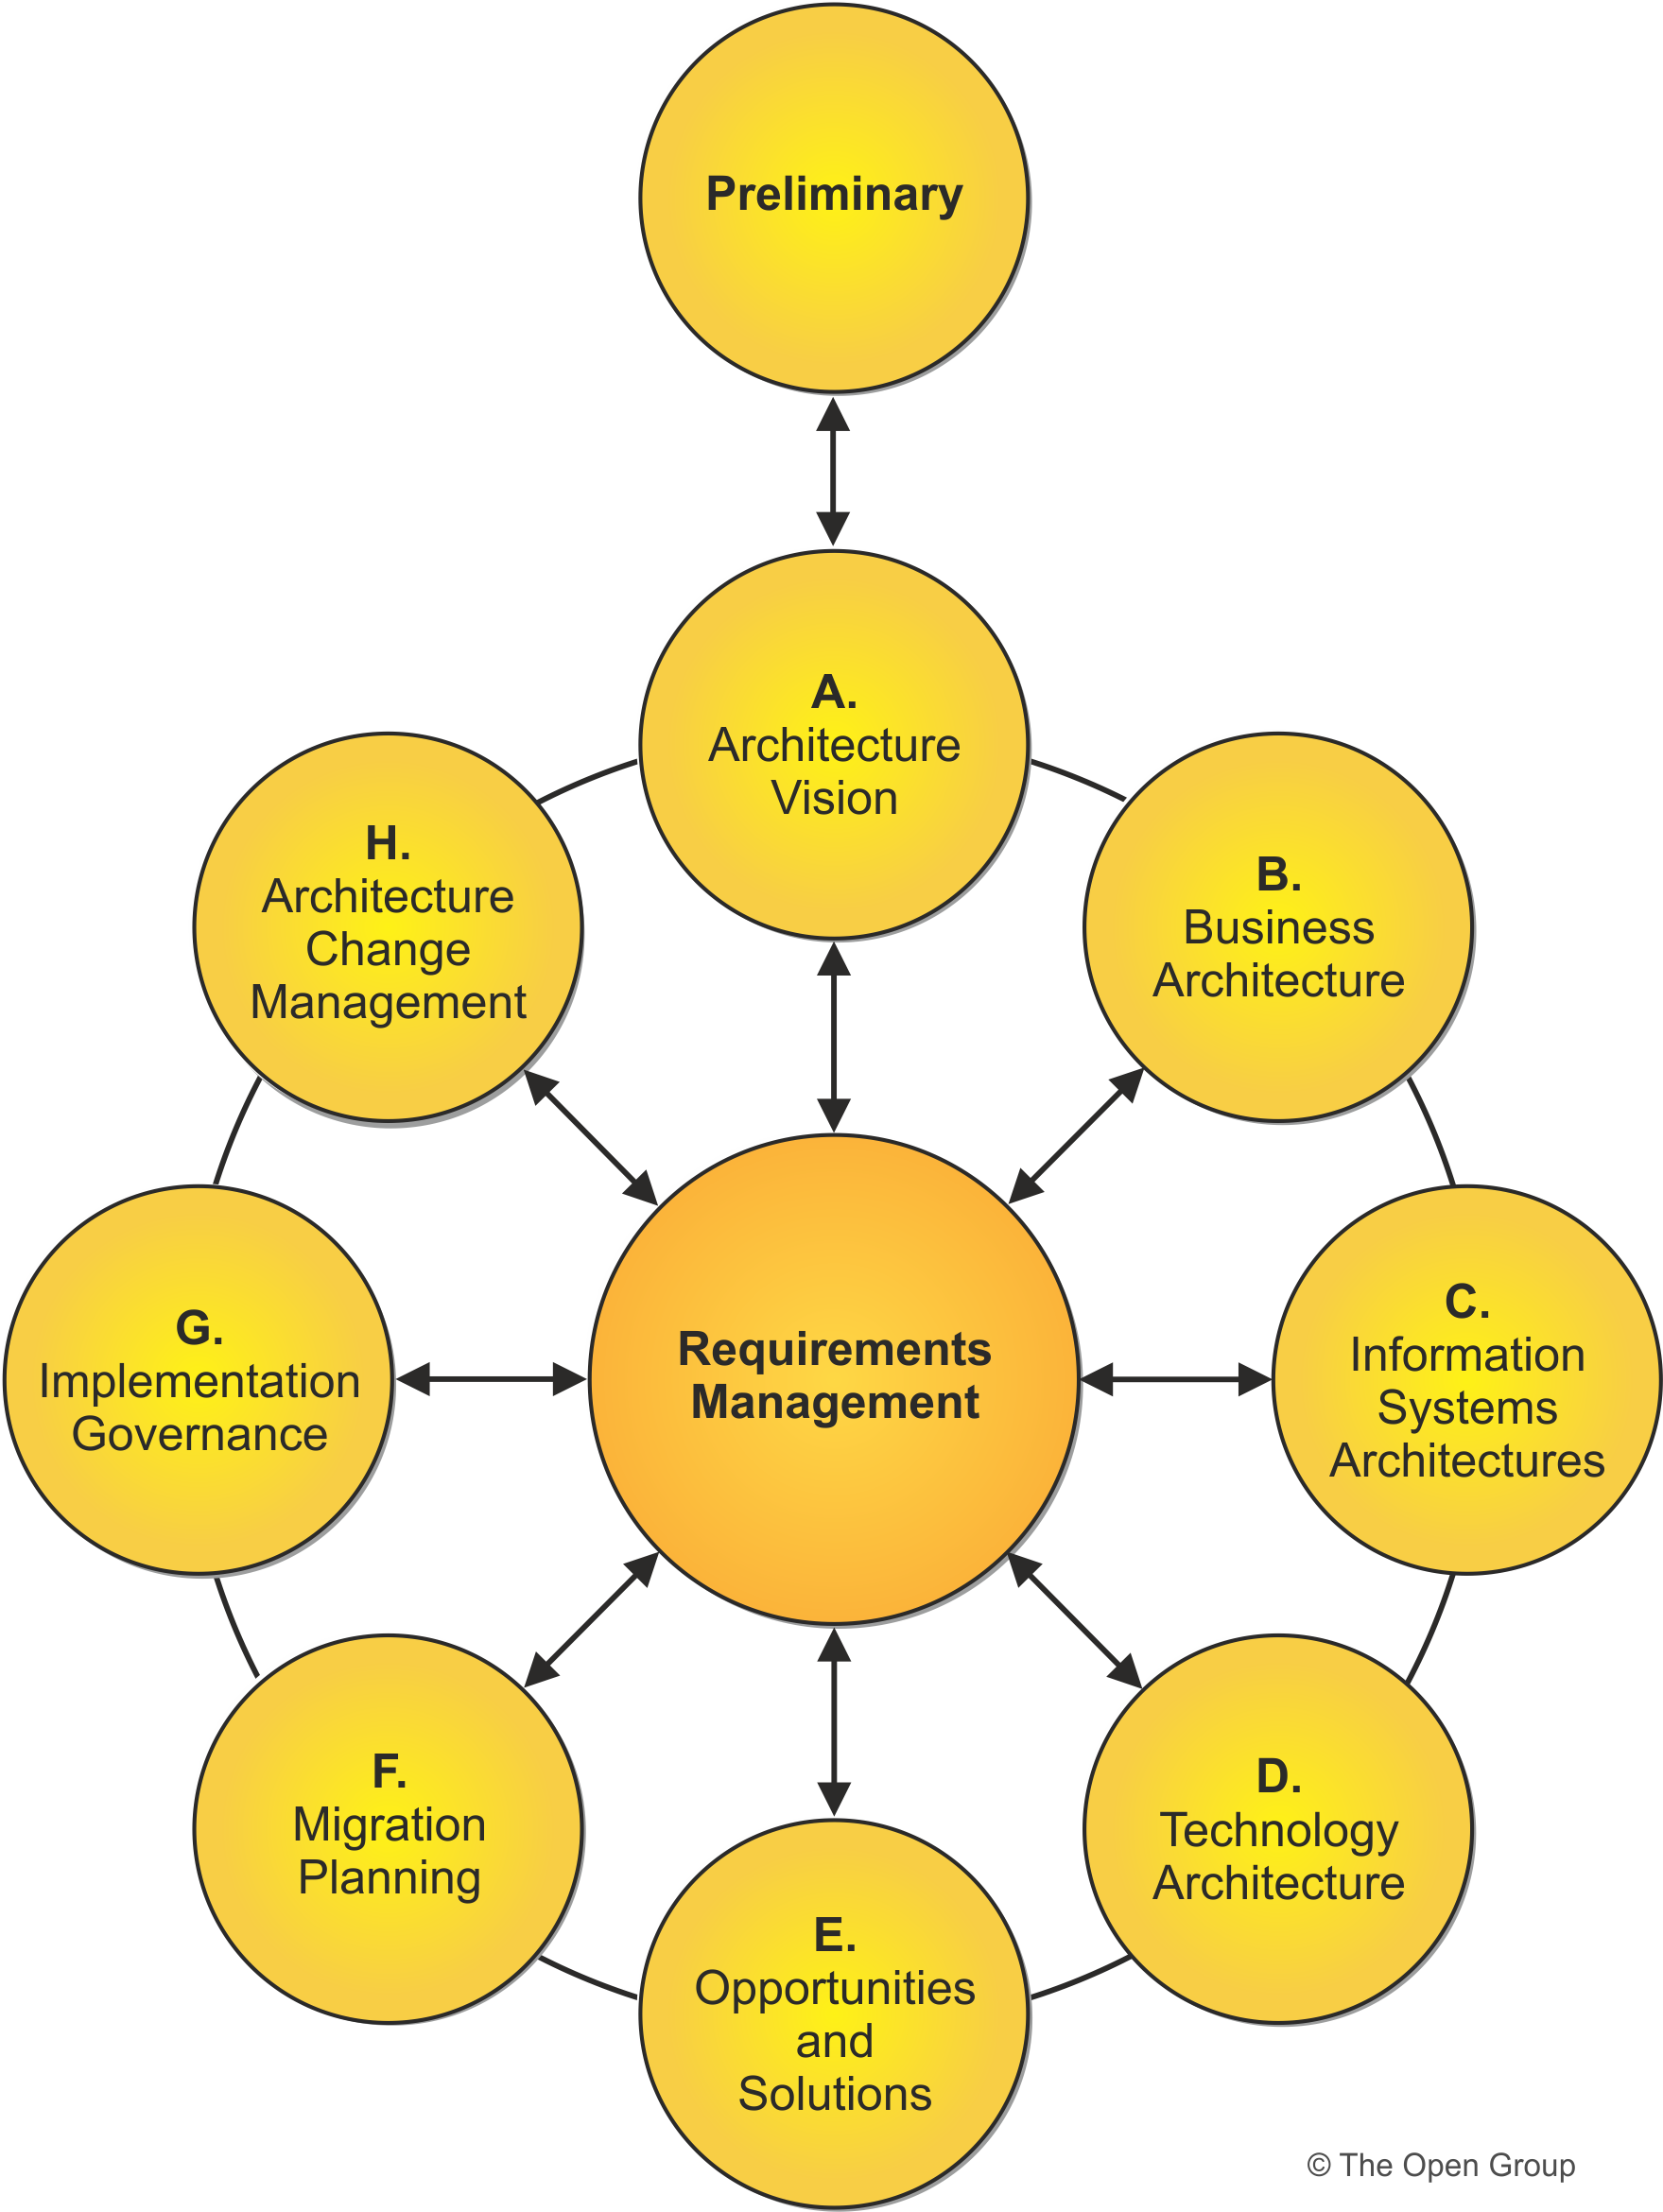
\includegraphics[width=0.38\textwidth]{../figures/adm}
			\end{center}
		\end{frame}
	}
	
	
	\begin{frame}
		\frametitle{Aims}
		\begin{enumerate}
			\item Ensure that the Requirements Management process is sustained and operates for all relevant ADM phases
			\item Manage architecture requirements identified during any execution of the ADM cycle or a phase
			\item Ensure that relevant architecture requirements are available for use by each phase as the phase is executed
		\end{enumerate}
		
	\end{frame}
	
		\begin{frame}
		\frametitle{Inputs}
		\vspace{20pt}
		\begin{enumerate}
			\item Inputs to Requirements Management process: Requirements-related outputs from each ADM phase.
			\item Initial high-level requirements: Produced during Architecture Vision phase.
			\item Detailed requirements: Generated by each architecture domain.
			\item Later phase deliverables: Include mappings to new types of requirements (e.g., conformance requirements).
		\end{enumerate}
	\end{frame}
	
	\begin{frame}
		\frametitle{Steps (1)}
		\vspace{20pt}
		\begin{enumerate}
			\item Identify/document requirements – use Business Scenarios or other techniques
			\begin{enumerate}
				\item Gap Analysis in ADM Phases B to D identifies gaps between Baseline and Target Architectures can lead to gap requirements.
			\end{enumerate}
			\item Create baseline requirements:
			\begin{enumerate}
				\item Determine priorities from the current phase of ADM.
				\item Confirm stakeholder agreement with resulting priorities.
				\item Record requirements priorities and save them in the Requirements Repository.
			\end{enumerate}
			\item Monitor baseline requirements
			 \item During ADM phases, identify changed requirements:
			\begin{enumerate}
				\item Remove or re-assess priorities
				\item Add requirements and re-assess priorities
				\item Modify existing requirements
			\end{enumerate}
		\end{enumerate}
	\end{frame}
	
	\begin{frame}
		\frametitle{Steps (2)}
		\vspace{20pt}
		\begin{enumerate}
			\setcounter{enumi}{4}
			\item In the baseline requirements, update changed requirements and record priorities:
			\begin{enumerate}
				\item Identify changed requirements. Prioritize them by responsible architects and stakeholders.
				\item Record new priorities.
				\item Identify and manage conflicts across phases.
				\item Generate Requirements Impact Statement for guiding the architecture team.
				\item \textbf{Note}:
				\begin{enumerate}
					\item Changed requirements from various sources.
					\item Process guides assessment and prioritization of requirements, aligning with ADM phases and documenting decisions.
					\item Requirements Management phase assesses stakeholder satisfaction.
					\item Dissatisfaction leads to issue resolution and determination of subsequent actions.
				\end{enumerate}
			\end{enumerate}
		\end{enumerate}
	\end{frame}
	
	\begin{frame}
		\frametitle{Steps (3)}
		\vspace{20pt}
		\begin{enumerate}
			\setcounter{enumi}{5}
			\item Analyze the impact of requirements changes:
			\begin{enumerate}
				\item Assess impact of changed requirements on the current (active) phase.
				\item Assess impact of changed requirements on previous phases.
				\item Decide whether to implement changes or postpone to a later ADM cycle.
				\item If implementing, evaluate the timescale for change management implementation.
				\item Issue Requirements Impact Statement, Version n+1.
			\end{enumerate}
			\item Implement Phase H requirements that can be fullfilled in that phase:
			\begin{enumerate}
				\item Architecture Change Management (Phase H) enables architecture changes throughout its lifecycle.
				\item Requirements Management handles new or changing requirements derived from Phase H.
			\end{enumerate}
					\item Update the Requirements Repository
			with information relating to the changes
			requested, including stakeholder views
			affected.
		\end{enumerate}
	\end{frame}


	\begin{frame}
		\frametitle{Outputs}
		\vspace{22pt}
		\begin{enumerate}
			\item Updated Architecture Requirements Specification
			\item Requirements Impact Assessment
		\end{enumerate}
	\end{frame}
	
	\begin{frame}
		\frametitle{Requirements Impact Assessment (1)}
		\vspace{22pt}
		\begin{enumerate}
			\item New information collected throughout ADM regarding architecture.
			\item New facts may invalidate existing aspects due to new/changed requirements.
			\item Requirements Impact Assessment: Evaluates current architecture requirements and identifies needed changes.
			\item Documented assessment and recommendations for architecture changes.
			\item Iterative process with final version encompassing full implications (costs, timescales, metrics).
		\end{enumerate}
		
	\end{frame}

	\begin{frame}
		\frametitle{Requirements Impact Assessment (2)}
		\vspace{22pt}
		\begin{enumerate}
			\item Recommended contents include specific requirements, stakeholder priorities, revisited phases, lead phase for prioritization, investigation results, management recommendations, repository reference.
			\item Often generated in response to Change Requests.
		\end{enumerate}
		
	\end{frame}
	
	\begin{frame}
		\frametitle{Summary}
		\begin{enumerate}
			\item Requirements Management: Ongoing activity in ADM.
			\item Requirements Repository: Holds current Target Architecture requirements.
			\item New/changed requirements: Trigger Requirements Impact Statement.
			\item Requirements Impact Statement: Identifies revisiting phases in ADM for addressing changes.
		\end{enumerate}
	\end{frame}
	
\end{document}
